\chapter{Sets and Mappings}
\section{Sets}
\begin{definition}{\quad Set}{def_2_1_1}
A \textbf{set} refers to a group of specific or abstract objects that share certain properties.
\end{definition}
\begin{definition}{\quad Elements}{def_2_1_2}
    The objects within a set are called the \textbf{elements} of the set.
\end{definition}

\begin{note}
    A \textbf{set} is typically denoted by a capital letter, such as $S$, while an \textbf{element} of the set is denoted by a lowercase letter, such as $s$. If $x$ is an element of a set $X$, then we write $x \in X$. Here, the symbol $\in$ means "is an element of" and is read as "in". If $x$ is not an element of a set $X$, then we write $x \notin X$. Here, the symbol $\notin$ means "is not an element of" and is read as "not in".
\end{note}

\begin{example}{}{exp_2_1_1}
    Lets see some common examples of sets:

    \begin{enumerate}[label=$\bullet$,topsep=10pt, itemsep=5pt]
        \item The set of integers: $\mathbb{Z} = \left\{0, \pm1, \pm2, \pm3, \dots \right\}$. 
        \item The set of rational numbers: $\mathbb{Q} = \left\{\frac{a}{b}:\, a,b \in \mathbb{Z}, b\neq0 \right\}$.
        \item The set of real numbers: $\mathbb{R}$.
        \item The set of complex numbers: $\mathbb{C} = \left\{ a+b\sqrt{-i} \mid a,b \in \mathbb{R} \right\}$.
        \item The empty set: $\emptyset$. There is no element in the set.
    \end{enumerate}
\end{example}

We uses two set representations:

\textbf{Roster Method}, which lists all the elements of the set explicitly, i.e., 
\[
\mathbb{Z} = \left\{0, \pm1, \pm2, \pm3, \dots \right\},
\]
and \textbf{Set-Builder Notation}, which defines the set by describing the properties or rules that its elements satisfy, i.e., 
\[
\mathbb{C} = \left\{ a+b\sqrt{-i} \mid a,b \in \mathbb{R} \right\}. 
\]

\begin{note}
    \begin{itemize}
        \item[1.] There is no order relationship in the representation of a set. That is $\left\{ x, y \right\} = \left\{y, x \right\}$. 
        \item[2.] Repetition of elements in a set is meaningless. That is $\left\{ x, y \right\} = \left\{y, x \right\} = \left\{x, y, x \right\} = \left\{x, y, x, x \right\}$. 
    \end{itemize}
\end{note}

\begin{definition}{\quad Subset}{def_2_1_3}
    Suppose $X$ and $Y$ are two sets, if every element of $X$ is an element of $Y$, that is
    \[
    x \in X \Rightarrow x \in Y, 
    \] 
    then we say $X$ is a \textbf{subset} of $Y$ and we denote this as $X \subseteq Y$.
\end{definition}

\begin{note}
    The $\Rightarrow$ symbol means "imply" and reads "if ... then ...".
\end{note}


\begin{example}{}{exp_2_1_2}
    Suppose we have a set $T = \left\{1, 2, 3 \right\}$, then $T$ has $2^{3}$ subsets:
    \begin{align*}
        &\emptyset; \\
        &\{1\}, \{2\}, \{3\}; \\
        &\{1,2\}, \{1,3\}, \{2,3\}; \\
        &\{1,2,3\}.
    \end{align*}
\end{example}
If there exists at least one $x \in X$ such that $x \notin Y$, then $X$ is not a subset of $Y$. We denote it as $X \not\subseteq Y$.

\begin{definition}{\quad Proper subset}{def_2_1_4}
    If $X$ is a subset of $Y$, but $X \neq Y$, then we say $X$ is a \textbf{proper subset} of $Y$ and we denote it as 
    \[
    X \subset Y.
    \]
\end{definition}

\begin{example}{}{exp_2_1_3}
    \[
    \mathbb{Z} \subset \mathbb{Q} \subset \mathbb{R}
    \]
\end{example}

\begin{example}{}{exp_2_1_4}
    If a set $T = \left\{t_{1}, t_{2}, t_{3}, \dots, t_{n} \right\}$, then set $T$ has $2^{n}$ subsets (including the empty set and the set itself) and $2^{n}-1$ proper subsets.
\end{example}

If all the elements of $X$ and $Y$ are the same, then we say $X$ and $Y$ are equal, denoted as $X=Y$. That is
\[
X = Y \iff X \subseteq Y \quad \text{and} \quad Y \subseteq X.
\]

\begin{note}
The $\iff$ symbol means "if and only if" and is read as "is equivalent to" or "exactly when".
\end{note}

\subsection{Set Operations}
We will introduce five common set operations, including: Union $(\cup)$, Intersection $(\cap)$, Difference $(\backslash)$, Complement $(^{c})$, and Cartesian Product $(\times)$. 

Suppose we have two sets $X$ and $Y$:
\begin{enumerate} 
    \item[1.] The \textbf{union} of two sets $X$ and $Y$ refers to the combination of all elements from both sets.  
    \[
    X \cup Y = \left\{x \mid x \in X \, \text{or} \, x \in Y\right\}
    \]
    \begin{center}
        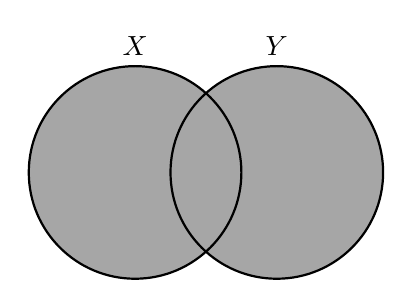
\begin{tikzpicture}[scale=.9]
            \def\radius{1.5}
            \def\distance{1}
            \coordinate (CenterX) at (-\distance, 0);
            \coordinate (CenterY) at (\distance, 0);
            \fill[gray!70] (CenterX) circle (\radius);
            \fill[gray!70] (CenterY) circle (\radius);
            \draw[thick] (CenterX) circle (\radius) node[anchor=south] at (-\distance, \radius) {$X$};
            \draw[thick] (CenterY) circle (\radius) node[anchor=south] at (\distance, \radius) {$Y$};
        \end{tikzpicture}
    \end{center}


    \item[2.] The \textbf{intersection} of two sets $X$ and $Y$ refers to the elements that are common to both sets.
    \[
    X \cap Y = \left\{x \mid x \in X \, \text{and} \, x \in Y \right\}
    \]
    \begin{center}
        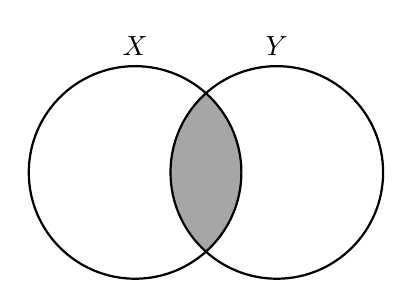
\begin{tikzpicture}[scale=.9]
            \def\radius{1.5}
            \def\distance{1}
            \coordinate (CenterX) at (-\distance, 0);
            \coordinate (CenterY) at (\distance, 0);
            \begin{scope}
                \clip (CenterX) circle (\radius);
                \fill[gray!70] (CenterY) circle (\radius);
            \end{scope}
            \draw[thick] (CenterX) circle (\radius) node[anchor=south] at (-\distance, \radius) {$X$};
            \draw[thick] (CenterY) circle (\radius) node[anchor=south] at (\distance, \radius) {$Y$};
        \end{tikzpicture}
    \end{center}
    
    The union and intersection of sets satisfy certain operational laws:
    \begin{enumerate}
        \item[a.] Commutative Law:
            \begin{align*}
                A \cup B &= B\cup A \\
                A \cap B &= B \cap A
            \end{align*}
        \item[b.] Associative Law:
            \begin{align*}
                A \cup (B \cup C) &= (A \cup B) \cup C \\
                A \cap (B \cap C) &= (A \cap B) \cap C
            \end{align*}
        \item[c.] Distributive Law:
            \begin{align*}
                A \cup (B\cap C) &= (A \cup B) \cap (A \cup C) \\
                A \cap (B \cup C) &= (A \cap B) \cup (A \cap C)
            \end{align*}
    \end{enumerate}

\begin{example}{}{ex_2_1_5}
For sets $A, B$, and $C$, prove the distributive law that is to show $A \cap (B \cup C) = (A \cap B) \cup (A \cap C)$. 
\end{example}
\begin{proof}{MyExpColor}
    To show $A \cap (B \cup C) = (A \cap B) \cup (A \cap C)$, first we need to show $A \cap (B \cup C) \subseteq (A \cap B) \cup (A \cap C)$. Second we need to show $(A \cap B) \cup (A \cap C) \subseteq A \cap (B \cup C)$.
    
    \noindent Step $1$: Show $x \in A \cap (B \cup C) \Rightarrow x \in (A\cap B)\cup(A \cap C) \iff A \cap (B \cup C) \subseteq (A\cap B)\cup (A \cap C)$ 
    \begin{align*}
        x \in A \cap (B \cup C) &\Rightarrow \\
        x \in A \text{ and } x \in (B \cup C) &\Rightarrow \\
        x \in A \text{ and } (x \in B \text{ or } x \in C) &\Rightarrow \textcolor{gray}{\text{x in A for sure (no graph)}}  \\
        (x \in A \text{ and } x \in B) \text{ or } (x \in A \text{ and } x \in C) & \Rightarrow \textcolor{gray}{\text{think it as two possibilities}} \\
        \text{(x in A and x in B) or (x in A and x in C)} &\Rightarrow (A\cap B)\cup (A \cap C)
    \end{align*}
    
    Therefore, we have $A \cap (B \cup C) \subseteq (A\cap B)\cup (A \cap C)$.

    \noindent Step $2$: Show $x \in (A\cap B)\cup(A \cap C) \Rightarrow x \in A \cap (B \cup C) \iff (A\cap B)\cup(A \cap C) \subseteq A \cap (B \cup C) $ 
    \begin{align*}
        x \in (A\cap B)\cup(A \cap C) &\Rightarrow \\ 
        \text{(x in A and x in B) or (x in A and x in C)} &\Rightarrow \textcolor{gray}{\text{graph}} \\
        \text{x in A and (x in B or x in C)} &\Rightarrow x \in A \cap (B \cup C)
    \end{align*}

    Therefore, we have $(A\cap B)\cup (A \cap C) \subseteq A \cap (B \cup C)$

    Thus, $A \cap (B \cup C) = (A \cap B) \cup (A \cap C)$.
\end{proof}

\item[3.] The \textbf{difference} of two sets $X$ and $Y$ refers to the set of elements that are in $X$ but not in $Y$. That is
\[
X \backslash Y = \left\{x \mid x\in X \text{ and } x \not\in Y \right\}.
\]

\begin{center}
    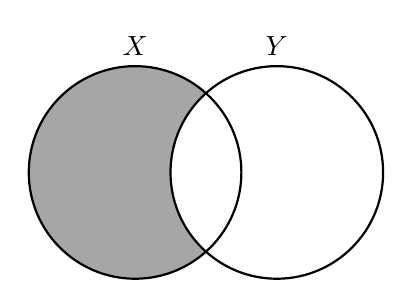
\begin{tikzpicture}[scale=.9]
        \def\radius{1.5}
        \def\distance{1}
        \coordinate (CenterX) at (-\distance, 0);
        \coordinate (CenterY) at (\distance, 0);
        \fill[gray!70] (CenterX) circle (\radius);
        \fill[white] (CenterY) circle (\radius); 
        \draw[thick] (CenterX) circle (\radius) node[anchor=south] at (-\distance, \radius) {$X$};
        \draw[thick] (CenterY) circle (\radius) node[anchor=south] at (\distance, \radius) {$Y$};
    \end{tikzpicture}
\end{center}

\noindent Note: here $X$ does not need to be a subset of $Y$. For example, if $X = \left\{ 1, 2, 3\right\}$ and $Y = \{ 3, 4, 5\}$, then $X\backslash Y = \{1,2\}$.

\item[4.] The \textbf{complement} of a set $X$ is the set of all elements in the universal set $U$ that are not in $X$. That is
\[
X^{c} = \{x \mid x \in U \text{ and } x \not\in X\} = U \backslash X.
\]
    \begin{center}
        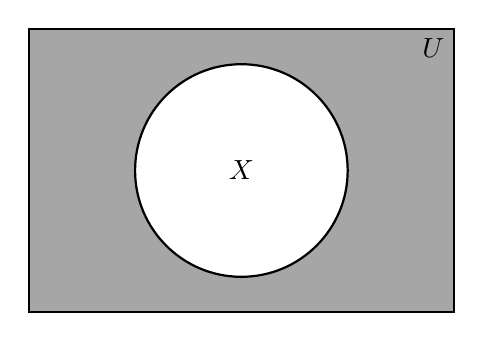
\begin{tikzpicture}[scale=.9]
            \def\boxwidth{6}
            \def\boxheight{4}
            \def\radius{1.5}
            \coordinate (CenterX) at (0, 0);
            \fill[gray!70] (-\boxwidth/2, -\boxheight/2) rectangle (\boxwidth/2, \boxheight/2);
            \draw[thick] (-\boxwidth/2, -\boxheight/2) rectangle (\boxwidth/2, \boxheight/2);
            \fill[white] (CenterX) circle (\radius); 
            \draw[thick] (CenterX) circle (\radius);
            \node at (CenterX) {$X$};
            \node[anchor=north east] at (\boxwidth/2, \boxheight/2) {$U$};
        \end{tikzpicture}
    \end{center}
\textbf{De Morgan Rule}: 
\begin{align*}
    (A \cup B)^{c} &= A^{c} \cap B^{c} \\
    (A \cap B)^{c} &= A^{c} \cup B^{c}
\end{align*}
\end{enumerate}



\subsection{Finite and Infinite Sets}
\begin{definition}{}{def_2_1_5}
    If a set $X$ consists of $n$ elements, where $n$ is a fixed non-negative integer, then $X$ is called a \textbf{finite set}. A set that is not finite is called an \textbf{infinite set}.
\end{definition} 

\begin{example}{}{}
    For example, $X = \{1,2,3\}, Y= \{y_{1}, y_{2}, y_{3}, \dots, y_{99}\}, \emptyset$ are finite sets, , while, $\mathbb{Q}, \mathbb{R}$ are infinite sets.
\end{example}

\begin{definition}{}{def_2_1_6}
      An infinite set is called a \textbf{countable set} if its elements can be arranged in a sequence according to some rule.
\end{definition}  

\begin{example}{}{exp_2_1_7}
    For example, $\mathbb{N} = \{1, 2, 3, \dots\}$ and $\{x \mid x = n\pi, n \in \mathbb{N}\}$ are countable sets.
\end{example}

\begin{note}
    It is obvious that any infinite set must contain a countable subset (proof required), but an infinite set is not necessarily countable. (In later course, we will show that $\mathbb{R}$ is an uncountable set.)
\end{note} 

Clearly, to prove that an infinite set is countable, the key is to design a rule for arranging the elements in such a way that all elements of the set can be listed without \underline{repetition} or \underline{omission}.

\begin{example}{}{def_2_1_8}
    Show that $\mathbb{Z}$ is a countable set.
\end{example}
\begin{proof}{MyExpColor}
    We can list $\mathbb{Z}$ as 
    \[
    \mathbb{Z} = \{0, \pm1, \pm,2, \pm3, \dots, \pm n, \dots\}, \quad n \in \mathbb{N}.
    \]
    Following this rule, we know that all elements in $\mathbb{Z}$ are listed without repetition or omission. Therefore $\mathbb{Z}$ is a countable set.
    \textcolor{gray}{
    \[
    \mathbb{Z} = \{\dots, -3, -2, -1, 0, 1, 2, 3, \dots \}
    \]
    }
\end{proof}

\begin{example}{}{def_2_1_9}
    Suppose we have $n \in \mathbb{N}$ number of countable sets, $A_{n}$. We have an important countable set built from these $A_{n}$. That is
    \begin{align*}
        \bigcup\limits_{n=1}^{\infty} A_{n} = A_{1} \cup A_{2} \cup \dots \cup A_{n} \cup \dots = \left\{x \mid \textcolor{red}{\exists} \, n \in \mathbb{N}^{+}, \text{ such that } x \in A_{n} \right\}
    \end{align*}
    In other words, we want to prove that the union of countably many countable sets is also countable.
\end{example}

\begin{theorem}{}{thm_2_1_1}
    The union of countably many countable sets is also countable.
\end{theorem}
\begin{proof}{MyThmColor}
    For any $n \in \mathbb{N}$, since $A_{n}$ is a countable set, then W.O.L.G, we can list $A_{n}$ as $A_{n} = \{a_{x1}, a_{x2}. \dots, a_{xk}, \dots\}$, for $k \in \mathbb{N}$. That is we have 
    \[
    \begin{array}{c @{\hspace{2\tabcolsep}} *{6}{c}}
        A_{1} & : & a_{11} & a_{12} & a_{13} & a_{14} & \dots \\
        A_{2} & : & a_{21} & a_{22} & a_{23} & a_{24} & \dots \\
        A_{3} & : & a_{31} & a_{32} & a_{33} & a_{34} & \dots \\
        A_{4} & : & a_{41} & a_{42} & a_{43} & a_{44} & \dots \\
        \vdots & : & \vdots  & \vdots  & \vdots  & \vdots   & \ddots  
    \end{array}
    \]
    
    There are various ways to list the elements in a sequence, one commonly used method is the \textbf{diagonalization method}. That is
    \[
    \bigcup\limits_{n=1}^{\infty} A_{n} = \left\{x_{11}, x_{12}, x_{21}, x_{13}, x_{22}, x_{31}, x_{14}, x_{23}, x_{32}, x_{41}, \dots \right\}.
    \]
    
    By listing the elements this way, we ensure that there is no omission. For different sets $A_{i}$ and $A_{j}$, with $i \neq j$, the intersection of $A_{i}$ and $A_{j}$ may not be the empty set. Therefore, we might have repetitions. We set the rule that if there is a repetition, we only include it once to ensure no duplicates.
\end{proof}

\begin{theorem}{}{thm_2_1_2}
    The set of rationals, $\mathbb{Q}$, is a countable set.
\end{theorem}
\begin{proof}{MyThmColor}
    The goal is to show that each element in $\mathbb{Q}$ is included and each element in $\mathbb{Q}$ is shown only once. 
    We want to show that $(-\infty, \infty)$ is a composite of countably many, $(n, n+1], n \in \mathbb{Z},$ small intervals. Therefore, we only need to show that all rational numbers in $(0, 1]$ is countable. Then we apply Theorem theorem 1.1.1 to complete the proof. 
    
    Each rational number in $\mathbb{Q}$ can be represented by $\frac{q}{p}$ with $p, q \in \mathbb{N}$, $p$ and $q$ are co-prime, and $q \leq p$. 
    
    For $p=1$, we have $x_{11} = \frac{1}{1}=1$ 
    
    For $p=2$, we have $x_{21} = \frac{1}{2}$ 
    
    \indent For $p=3$, we have $x_{31} = \frac{1}{3}, x_{32} = \frac{2}{3}$ 
    
    \indent For $p=4$, we have $x_{41} = \frac{1}{4}, x_{42} = \frac{3}{4}$ \textcolor{gray}{\text{ensure no repetition}} 
    
    \indent $\vdots$ 
    
    \indent For $p=n$, we have $x_{n1} = \frac{1}{n}, x_{n2}, \dots, x_{nk(n)}$ \textcolor{gray}{\text{ensure no repetition}} 
    
    \indent $\vdots$ 
    
    Therefore, all rationals in $(0,1]$ can be listed as $x_{11}, x_{21}, x_{31}, x_{32}, x_{41}, x_{42}, \dots, x_{n1}, x_{n2}, \dots, x_{nk(n)}$. This way we ensure that each element is included and each element is shown only once. 
\end{proof}



\subsection{Cartesian Product of Sets}
\begin{definition}{}{def_2_1_7}
    Let $X$ and $Y$ be two sets. For any element $x$ chosen from set $X$ and any element $y$ chosen from set $Y$, the ordered pair $(x, y)$ is formed. The collection of all such ordered pairs is called the \textbf{Cartesian product} of sets of $X$ and $Y$. That is
    \[
    X \times Y = \left\{(x,y) \mid x\in X \text{ and } y \in Y \right\}.
    \]
\end{definition}

\begin{example}{}{}
    A special case is when $A=B=\mathbb{R}$, in which case we have the \textbf{Cartesian coordinate system in two dimensions}, $\mathbb{R}^{2} = \mathbb{R} \times \mathbb{R}$. The \textbf{Cartesian coordinate system in three dimensions} is $\mathbb{R}^{3} = \mathbb{R}\times\mathbb{R}\times\mathbb{R}$.
\end{example}

\begin{example}{}{}
    Say we have $A = \left\{ x \,|\, a \leq x \leq b \right\}$, $B = \left\{ y \,|\, c \leq y \leq d \right\}$, and $C = \left\{ z \,|\, e \leq z \leq f \right\}$, then $A \times B$ is composite of all points in a rectangle.
    \begin{figure}[H]
        \begin{center}
        \definecolor{ududff}{rgb}{0.30196078431372547,0.30196078431372547,1}
            \resizebox{0.6\textwidth}{!}{
            \begin{tikzpicture}[line cap=round,line join=round,>=triangle 45,x=1cm,y=1cm]
            \begin{axis}[
                x=1cm,y=1cm,
                axis lines=middle,
                ymajorgrids=true,
                xmajorgrids=true,
                xmin=-2.38,
                xmax=6.38,
                ymin=-2.38,
                ymax=4.38,
                xtick={-7,-6,...,15},
                ytick={-5,-4,...,7},
                % --- NEW OPTIONS TO MOVE TICK LABELS ---
                xticklabel style={yshift=-5pt}, % Moves X labels 5pt down
                yticklabel style={xshift=-5pt}, % Moves Y labels 5pt left
                % -----------------------------------------
                ]
                \clip(-7.38,-5.77) rectangle (15.58,7.05);
                \draw [line width=2pt] (2,3)-- (2,1);
                \draw [line width=2pt] (2,1)-- (5,1);
                \draw [line width=2pt] (5,1)-- (5,3);
                \draw [line width=2pt] (5,3)-- (2,3);
                \begin{scriptsize}
                \draw [fill=ududff] (2,0) circle (2.5pt);
                \draw[color=ududff] (2.16,0.42) node {$a$};
                \draw [fill=ududff] (5,0) circle (2.5pt);
                \draw[color=ududff] (5.16,0.42) node {$b$};
                \draw [fill=ududff] (0,1) circle (2.5pt);
                \draw[color=ududff] (0.16,1.42) node {$c$};
                \draw [fill=ududff] (0,3) circle (2.5pt);
                \draw[color=ududff] (0.16,3.42) node {$d$};
                \end{scriptsize}
            \end{axis}
            \end{tikzpicture}
            }
        \end{center}
    \end{figure}

    It is easy to know that $A \times B \times C$ are all points in a cuboid.
\end{example}



\subsection{Exercises}
\begin{question}
    Prove that the set $T = \left\{t_{1}, t_{2}, \dots, t_{n}\right\}$ has $2^{n}$ subsets.
\end{question}
\begin{proof}{}
    We prove the statement by listing subsets with $0, 1, \dots, n$ elements and add them up. 
    \begin{enumerate}
        \item[] There is $\Comb{n}{0}$ subset with $0$ element: $\emptyset$, 
        \item[] There are $\Comb{n}{1}$ subsets with $1$ elements: $\{t_{1}\}, \{t_{2}\}, \dots, \{t_{n}\}$,
        \item[] There are $\Comb{n}{2}$ subsets with $2$ elements,
        \item[] $\dots$
        \item[] There are $\Comb{n}{k}$ subsets with $k$ elements, with $k \in \mathbb{N}$,
        \item[] $\dots$
        \item[] There is $\Comb{n}{n}$ subset with $n$ elements: $T$.
    \end{enumerate}
    
    Therefore the total number of subsets is $\Comb{n}{0} + \Comb{n}{1} + \Comb{n}{2} + \dots + \Comb{n}{k} + \dots + \Comb{n}{n} = \sum\limits_{k=0}^{n}\binom{n}{k}$. Recall that the binomial theorem states that 
    \[
    (a+b)^{n} = \sum\limits_{k=0}^{n}\binom{n}{k}a^{n-k}b^{k}.
    \]
    
    It is obvious that by setting $a=b=1$ we have that $2^{n} = \sum\limits_{k=0}^{n}\binom{n}{k}$.
\end{proof}

\begin{question}
    Prove: 
    
    $1.$ Any infinite set must have a countable subset.
    
    $2.$ Assume two sets $A$ and $B$ are countable sets, show that $A \cup B$ is a countable set.
\end{question}
\begin{proof}{}
    For $1$, 
\end{proof}



\section{Mappings}
\subsection{Mappings}
A \textbf{mapping} refers to the correspondence between sets.
\begin{definition}{}{}
     Let $X$ and $Y$ be two given sets. If there exists a rule $f$ such that for every element $x$ in the set $X$, a uniquely determined element $y$ in the set $Y$ can be found corresponding to it, then this rule $f$ is called a \textbf{mapping} from set $X$ to set $Y$. It is denoted as 
    \begin{align*}
        f: &X \rightarrow Y; \\
           &x \mapsto y =f(x).
    \end{align*}
\end{definition}

\begin{definition}{}{}
    If $f$ is a mapping from $X$ to $Y$. then $y$ is called the \textbf{image} of $x$ under the mapping $f$, and $x$ is called the \textbf{preimage} (or \textbf{inverse image}) of $y$ under the mapping $f$.
\end{definition}

\begin{definition}{}{}
    If $f$ is a mapping from $X$ to $Y$. The set $X$ is called the \textbf{domain} of the mapping $f$, denoted as $D_{f} = X$, and the set of all images $y$ of the elements $x$ in $X$ under the mapping $f$ is called the \textbf{range} of the mapping $f$, denoted as $R_{f} = \left\{ y \mid y \in Y \text{ and } y = f(x), \, \forall x \in X \right\}$, with $R_{f} \, \textcolor{red}{\subseteq}\, Y$. The set $Y$ consists of the possible outcome values under the mapping $f$, so $Y$ is called the \textbf{codomain} of the mapping $f$, denoted as $C_{f}$.
\end{definition}

\begin{note}
Three key elements of a mapping: 
\begin{enumerate}
    \item [1.] $X = D_{f}$;
    \item [2.] $Y = C_{f}$;
    \item [3.] $R_{f} \textcolor{red}{\subseteq} Y$;
    \item [4.] $f$ has the property: The \textbf{uniqueness of the image} and the \textbf{non-uniqueness of the preimage}. \textcolor{red}{The \textbf{uniqueness of the image} means that in the set $X$, any element cannot have more than one outgoing arrow.}
\end{enumerate}
\end{note}

\begin{example}{}{exp_2_2_1}
        \begin{center}
        \resizebox{0.8\textwidth}{!}{
            \begin{tikzpicture}[scale=1.5]
                \pgfmathsetmacro{\vsep}{0.4} 
                \pgfmathsetmacro{\starty}{0.5} 
                % Coordinates for Row 1
                \coordinate (C1) at (0, 0); 
                \coordinate (C2) at (2.5, 0); 
                \coordinate (C3) at (5, 0); 
                \coordinate (C4) at (7.5, 0); 
                % --- Diagram 1 (Upper Left: Surjective) ---
                \node[set] (X1) at (C1) {};
                \node[set] (Y1) at (C2) {};
                \node[above=0.2cm of X1.north] {$X$};
                \node[element] (x11) at ($(X1.north) + (0, -\starty)$) {};
                \node[element] (x12) at ($(x11) + (0, -\vsep)$) {};
                \node[element] (x13) at ($(x12) + (0, -\vsep)$) {};
                \node[element] (x14) at ($(x13) + (0, -\vsep)$) {};
                \node[left=0.1cm of x11] {$x_1$}; \node[left=0.1cm of x12] {$x_2$};
                \node[left=0.1cm of x13] {$x_3$}; \node[left=0.1cm of x14] {$x_4$};
                \node[element] (y11) at ($(Y1.north) + (0, -\starty)$) {};
                \node[element] (y12) at ($(y11) + (0, -\vsep)$) {};
                \node[element] (y13) at ($(y12) + (0, -\vsep)$) {};
                \node[element] (y14) at ($(y13) + (0, -\vsep)$) {};
                \node[right=0.1cm of y11] {$y_1$}; \node[right=0.1cm of y12] {$y_2$};
                \node[right=0.1cm of y13] {$y_3$}; \node[right=0.1cm of y14] {$y_4$};
                \node[above=0.05cm of Y1.north] {\color{blue}$Y = C_{f_{1}} = R_{f_{1}}$};
                \node[blue] at ($(Y1.east) + (-0.19, 0.08)$) {$R_{f_{1}}$};
                \draw[->] (x11) -- (y11); \draw[->] (x12) -- (y12);
                \draw[->] (x13) -- (y13); \draw[->] (x14) -- (y14);
                \node at ($(X1)!0.5!(Y1)$) [above=1.1cm] {$f_1$};
                \draw[dashed, blue, line width=1pt] ($(Y1.north east) + (-0.15, -0.01)$) rectangle ($(Y1.south west) + (0.3, 0.1)$); 
                \node at (1.25, -1.2) {a mapping};
                % --- Diagram 2 (Upper Right: Non-Surjective) ---
                \node[set] (X2) at (C3) {};
                \node[set] (Y2) at (C4) {};
                \node[above=0.2cm of X2.north] {$X$};
                \node[element] (x21) at ($(X2.north) + (0, -0.5)$) {};
                \node[element] (x22) at ($(x21) + (0, -\vsep)$) {};
                \node[element] (x23) at ($(x22) + (0, -\vsep)$) {};
                \node[element] (x24) at ($(x23) + (0, -\vsep)$) {};
                \node[left=0.1cm of x21] {$x_1$}; \node[left=0.1cm of x22] {$x_2$};
                \node[left=0.1cm of x23] {$x_3$}; \node[left=0.1cm of x24] {$x_4$};
                \node[element] (y21) at ($(Y2.north) + (0, -0.5)$) {};
                \node[element] (y22) at ($(y21) + (0, -\vsep)$) {};
                \node[element] (y23) at ($(y22) + (0, -\vsep)$) {};
                \node[element] (y24) at ($(y23) + (0, -\vsep)$) {};
                \node[right=0.1cm of y21] {$y_1$}; \node[right=0.1cm of y22] {$y_2$};
                \node[right=0.1cm of y23] {$y_3$}; \node[right=0.1cm of y24] {$y_4$};
                \node[above=0.1cm of Y2.north, align=center] {$Y = C_{f_{2}}$, \color{blue}$R_{f_{2}} \subset C_{f_{2}}$};
                \draw[->] (x21) -- (y21); \draw[->] (x22) -- (y22);
                \draw[->] (x23) -- (y23); \draw[->] (x24) -- (y23);
                \node at ($(X2)!0.5!(Y2)$) [above=1.1cm] {$f_2$};
                \draw[dashed, blue, line width=0.8pt] ($(Y2.north east) + (-0.15, -0.01)$) rectangle ($(Y2.south west) + (0.3, 0.5)$);
                \node[blue] at ($(Y2.east) + (-0.19, 0.08)$) {$R_{f_{2}}$};
                \node at (6.25, -1.2) {a mapping};
            \end{tikzpicture}
        }
        \resizebox{0.8\textwidth}{!}{
            \begin{tikzpicture}[scale=1.5]
                \pgfmathsetmacro{\vsep}{0.4} 
                \pgfmathsetmacro{\starty}{0.5} 
                % Coordinates reset for the "new" top row
                \coordinate (C5) at (0, 0); 
                \coordinate (C6) at (2.5, 0); 
                \coordinate (C7) at (5, 0); 
                \coordinate (C8) at (7.5, 0); 
                % --- Diagram 3 (Lower Left: NOT a mapping) ---
                \node[set] (X3) at (C5) {};
                \node[set] (Y3) at (C6) {};
                \node[above=0.2cm of X3.north] {$X$};
                \node[above=0.2cm of Y3.north] {$Y$};
                \node[element] (x31) at ($(X3.north) + (0, -0.5)$) {};
                \node[element] (x32) at ($(x31) + (0, -\vsep)$) {};
                \node[element] (x33) at ($(x32) + (0, -\vsep)$) {};
                \node[element] (x34) at ($(x33) + (0, -\vsep)$) {};
                \node[left=0.1cm of x31] {$x_1$}; \node[left=0.1cm of x32] {$x_2$};
                \node[left=0.1cm of x33] {$x_3$}; \node[left=0.1cm of x34] {$x_4$};
                \node[element] (y31) at ($(Y3.north) + (0, -0.5)$) {};
                \node[element] (y32) at ($(y31) + (0, -\vsep)$) {};
                \node[element] (y33) at ($(y32) + (0, -\vsep)$) {};
                \node[element] (y34) at ($(y33) + (0, -\vsep)$) {};
                \node[right=0.1cm of y31] {$y_1$}; \node[right=0.1cm of y32] {$y_2$};
                \node[right=0.1cm of y33] {$y_3$}; \node[right=0.1cm of y34] {$y_4$};
                \draw[->] (x31) -- (y31); \draw[->] (x32) -- (y32);
                \draw[->] (x33) -- (y33); \draw[->] (x34) -- (y33);
                \draw[->] (x34) -- (y34);
                \node at ($(X3)!0.5!(Y3)$) [above=1.1cm] {$f_3$};
                \node at (1.25, -1.25) {NOT a mapping};
                % --- Diagram 4 (Lower Right: NOT a mapping) ---
                \node[set] (X4) at (C7) {};
                \node[set] (Y4) at (C8) {};
                \node[above=0.2cm of X4.north] {$X$};
                \node[above=0.2cm of Y4.north] {$Y$};
                \node[element] (x41) at ($(X4.north) + (0, -0.5)$) {};
                \node[element] (x42) at ($(x41) + (0, -\vsep)$) {};
                \node[element] (x43) at ($(x42) + (0, -\vsep)$) {};
                \node[element] (x44) at ($(x43) + (0, -\vsep)$) {};
                \node[left=0.1cm of x41] {$x_1$}; \node[left=0.1cm of x42] {$x_2$};
                \node[left=0.1cm of x43] {$x_3$}; \node[left=0.1cm of x44] {$x_4$};
                \node[element] (y41) at ($(Y4.north) + (0, -0.5)$) {};
                \node[element] (y42) at ($(y41) + (0, -\vsep)$) {};
                \node[element] (y43) at ($(y42) + (0, -\vsep)$) {};
                \node[element] (y44) at ($(y43) + (0, -\vsep)$) {};
                \node[right=0.1cm of y41] {$y_1$}; \node[right=0.1cm of y42] {$y_2$};
                \node[right=0.1cm of y43] {$y_3$}; \node[right=0.1cm of y44] {$y_4$};
                \draw[->] (x41) -- (y41); \draw[->] (x42) -- (y42); \draw[->] (x44) -- (y44);
                \node at ($(X4)!0.5!(Y4)$) [above=1.1cm] {$f_4$};
                \node at (6.25, -1.25) {NOT a mapping};
            \end{tikzpicture}
        }
    \end{center}








 
    In the figure above, $f_{1}$ and $f_{2}$ are mapping since the uniqueness of image, while $f_{3}$ is not a mapping because the uniqueness of image is violated. Specifically, $x_{4}$ is mapped to two different elements in the set $Y$. In addition, $f_{4}$ is not a mapping since one of the element, $x_{3}$, in the set $X$ is not mapped to any element in the set $Y$.
\end{example}

\begin{example}{}{exp_2_2_2}
    Let $X = Y = \mathbb{R}$ and $f: X \rightarrow Y$ with $f(x) = x^{2}$. It should be obvious that $f$ is a mapping.
\end{example}
\begin{example}{}{}
    Let $X = \mathbb{R}^{+}, Y = \mathbb{R}$ with $f: X \rightarrow Y, x \mapsto y: y^{2} = x$. Then it is obvious that $f$ is not a mapping, since when $x = 4$, $y = \pm2$, meaning the image is not unique.
\end{example}
\begin{example}{}{}
    Let $X = \mathbb{R}^{+}, Y = \mathbb{R}^{-}$ with $f: X \rightarrow Y, x \mapsto y: y^{2} = x$. Then it is obvious that $f$ is a mapping.
\end{example}

\begin{definition}{}{}
    If $f$ is a mapping from $X$ to $Y$ and $f$ has the uniqueness of pre-image property, then we say $f$ is an \textbf{injection} or $f$ is \textbf{injective} (or \textbf{one-to-one}). To show $f$ is injective, we only need to show:
    \[
    x_{1} \neq x_{2} \Rightarrow f(x_{1}) \neq f(x_{2}).
    \]
\end{definition}
\begin{note}
    \begin{enumerate}
        \item[1.] For a mapping to be qualified as an injection, it needs to have the uniqueness property for the preimage. \\
        \textcolor{red}{The \textbf{uniqueness of the preimage} means that in the set $Y$, any element cannot have more than one ingoing arrow.}
        \item[2.] A mapping already has the uniqueness property for the image. So for a mapping to be a injection only uniqueness property for the preimage is needed.
    \end{enumerate}
\end{note}

\begin{example}{}{exp_2_2_5}
\begin{center}
    \resizebox{0.7\textwidth}{!}{
        \begin{tikzpicture}[scale=1.2, node distance=2.5cm and 2cm]
            \pgfmathsetmacro{\vsep}{0.4} 
            \pgfmathsetmacro{\starty}{0.8} 
            \coordinate (C1) at (0, 0); 
            \coordinate (C2) at (2.5, 0); 
            \coordinate (C3) at (5, 0); 
            \coordinate (C4) at (7.5, 0); 

            % --- Diagram 1 (g1) ---
            \node[set] (X1) at (C1) {}; \node[set] (Y1) at (C2) {};
            \node[above=0.2cm of X1.north] {$X$};
            \node[element] (x11) at ($(X1.north) + (0, -\starty)$) {};
            \node[element] (x12) at ($(x11) + (0, -\vsep)$) {};
            \node[element] (x13) at ($(x12) + (0, -\vsep)$) {};
            \node[element] (x14) at ($(x13) + (0, -\vsep)$) {};
            \node[left=0.1cm of x11] {$x_1$}; \node[left=0.1cm of x12] {$x_2$}; \node[left=0.1cm of x13] {$x_3$}; \node[left=0.1cm of x14] {$x_4$};
            \node[element] (y11) at ($(Y1.north) + (0, -\starty)$) {};
            \node[element] (y12) at ($(y11) + (0, -\vsep)$) {};
            \node[element] (y13) at ($(y12) + (0, -\vsep)$) {};
            \node[element] (y14) at ($(y13) + (0, -\vsep)$) {};
            \node[right=0.1cm of y11] {$y_1$}; \node[right=0.1cm of y12] {$y_2$}; \node[right=0.1cm of y13] {$y_3$}; \node[right=0.1cm of y14] {$y_4$};
            \node[above=0.1cm of Y1.north] {\color{blue}$Y = C_{g_{1}} = R_{g_{1}}$};
            \draw[->] (x11) -- (y11); \draw[->] (x12) -- (y12); \draw[->] (x13) -- (y13); \draw[->] (x14) -- (y14);
            \node at ($(X1)!0.5!(Y1)$) [above=1.1cm] {$g_1$};
            \draw[dashed, blue, line width=0.8pt] ($(Y1.north east) + (-0.2, -0.1)$) rectangle ($(Y1.south west) + (0.4, 0.2)$); 
            \node[blue] at ($(Y1.east) + (-0.25, 0.08)$) {$R_{g_{1}}$};
            \node at (1.25, -1.5) {an injection};

            % --- Diagram 2 (g2) ---
            \node[set] (X2) at (C3) {}; \node[set] (Y2) at (C4) {};
            \node[above=0.2cm of X2.north] {$X$};
            \node[element] (x21) at ($(X2.north) + (0, -\starty)$) {};
            \node[element] (x22) at ($(x21) + (0, -\vsep)$) {};
            \node[element] (x23) at ($(x22) + (0, -\vsep)$) {};
            \node[left=0.1cm of x21] {$x_1$}; \node[left=0.1cm of x22] {$x_2$}; \node[left=0.1cm of x23] {$x_3$};
            \node[element] (y21) at ($(Y2.north) + (0, -\starty)$) {};
            \node[element] (y22) at ($(y21) + (0, -\vsep)$) {};
            \node[element] (y23) at ($(y22) + (0, -\vsep)$) {};
            \node[element] (y24) at ($(y23) + (0, -\vsep)$) {};
            \node[right=0.1cm of y21] {$y_1$}; \node[right=0.1cm of y22] {$y_2$}; \node[right=0.1cm of y23] {$y_3$}; \node[right=0.1cm of y24] {$y_4$};
            \node[above=0.1cm of Y2.north, align=center] {$Y = C_{g_{2}}$, \color{blue}$R_{g_{2}} \subset C_{g_{2}}$};
            \draw[->] (x21) -- (y21); \draw[->] (x22) -- (y22); \draw[->] (x23) -- (y23);
            \node at ($(X2)!0.5!(Y2)$) [above=1.1cm] {$g_2$};
            \draw[dashed, blue, line width=0.8pt] ($(Y2.north east) + (-0.2, -0.1)$) rectangle ($(Y2.south west) + (0.4, 0.7)$); 
            \node[blue] at ($(Y2.east) + (-0.25, 0.08)$) {$R_{g_{2}}$};
            \node at (6.25, -1.5) {an injection};   
        \end{tikzpicture}
    }

    \resizebox{0.35\textwidth}{!}{ % Narrowed resizebox since it's only one diagram
        \begin{tikzpicture}[scale=1.2, node distance=2.5cm and 2cm]
            \pgfmathsetmacro{\vsep}{0.4} 
            \pgfmathsetmacro{\starty}{0.8} 
            % Reset origin to 0,0
            \coordinate (C_Mid_X) at (0, 0); 
            \coordinate (C_Mid_Y) at (2.5, 0); 

            % --- Diagram 3 (g3) ---
            \node[set] (X3) at (C_Mid_X) {}; \node[set] (Y3) at (C_Mid_Y) {};
            \node[above=0.2cm of X3.north] {$X$};
            \node[element] (x31) at ($(X3.north) + (0, -\starty)$) {};
            \node[element] (x32) at ($(x31) + (0, -\vsep)$) {};
            \node[element] (x33) at ($(x32) + (0, -\vsep)$) {};
            \node[element] (x34) at ($(x33) + (0, -\vsep)$) {};
            \node[left=0.1cm of x31] {$x_1$}; \node[left=0.1cm of x32] {$x_2$}; \node[left=0.1cm of x33] {$x_3$}; \node[left=0.1cm of x34] {$x_4$};
            \node[element] (y31) at ($(Y3.north) + (0, -\starty)$) {};
            \node[element] (y32) at ($(y31) + (0, -\vsep)$) {};
            \node[element] (y33) at ($(y32) + (0, -\vsep)$) {};
            \node[element] (y34) at ($(y33) + (0, -\vsep)$) {};
            \node[right=0.1cm of y31] {$y_1$}; \node[right=0.1cm of y32] {$y_2$}; \node[right=0.1cm of y33] {$y_3$}; \node[right=0.1cm of y34] {$y_4$};
            \node[above=0.1cm of Y3.north, align=center] {$Y = C_{g_{3}}$, \color{blue}$R_{g_{3}} \subset C_{g_{3}}$};
            \draw[->] (x31) -- (y31); \draw[->] (x32) -- (y32); \draw[->] (x33) -- (y33); \draw[->] (x34) -- (y33);
            \node at ($(X3)!0.5!(Y3)$) [above=1.1cm] {$g_3$};
            \draw[dashed, blue, line width=0.8pt] ($(Y3.north east) + (-0.2, -0.1)$) rectangle ($(Y3.south west) + (0.4, 0.7)$); 
            \node[blue] at ($(Y3.east) + (-0.25, 0.08)$) {$R_{g_{3}}$};
            \node[align=center] at (1.25, -1.75) {a mapping \\ NOT an injection};
        \end{tikzpicture}
    }

    \resizebox{0.7\textwidth}{!}{
        \begin{tikzpicture}[scale=1.2, node distance=2.5cm and 2cm]
            \pgfmathsetmacro{\vsep}{0.4} 
            \pgfmathsetmacro{\starty}{0.8} 
            % Reset origin to 0,0
            \coordinate (C7) at (0, 0); 
            \coordinate (C8) at (2.5, 0); 
            \coordinate (C9) at (5, 0); 
            \coordinate (C10) at (7.5, 0); 

            % --- Diagram 4 (g4) ---
            \node[set] (X4) at (C7) {}; \node[set] (Y4) at (C8) {};
            \node[above=0.2cm of X4.north] {$X$}; \node[above=0.2cm of Y4.north] {$Y$};
            \node[element] (x41) at ($(X4.north) + (0, -\starty)$) {};
            \node[element] (x42) at ($(x41) + (0, -\vsep)$) {};
            \node[element] (x43) at ($(x42) + (0, -\vsep)$) {};
            \node[element] (x44) at ($(x43) + (0, -\vsep)$) {};
            \node[left=0.1cm of x41] {$x_1$}; \node[left=0.1cm of x42] {$x_2$}; \node[left=0.1cm of x43] {$x_3$}; \node[left=0.1cm of x44] {$x_4$};
            \node[element] (y41) at ($(Y4.north) + (0, -\starty)$) {};
            \node[element] (y42) at ($(y41) + (0, -\vsep)$) {};
            \node[element] (y43) at ($(y42) + (0, -\vsep)$) {};
            \node[element] (y44) at ($(y43) + (0, -\vsep)$) {};
            \node[right=0.1cm of y41] {$y_1$}; \node[right=0.1cm of y42] {$y_2$}; \node[right=0.1cm of y43] {$y_3$}; \node[right=0.1cm of y44] {$y_4$};
            \draw[->] (x41) -- (y41); \draw[->] (x42) -- (y42); \draw[->] (x43) -- (y43); \draw[->] (x44) -- (y43); \draw[->] (x44) -- (y44);
            \node at ($(X4)!0.5!(Y4)$) [above=1.1cm] {$g_4$};
            \node[align=center] at (1.25, -2.0) {NOT a mapping \\ NOT an injection};

            % --- Diagram 5 (g5) ---
            \node[set] (X5) at (C9) {}; \node[set] (Y5) at (C10) {};
            \node[above=0.2cm of X5.north] {$X$}; \node[above=0.2cm of Y5.north] {$Y$};
            \node[element] (x51) at ($(X5.north) + (0, -\starty)$) {};
            \node[element] (x52) at ($(x51) + (0, -\vsep)$) {};
            \node[element] (x53) at ($(x52) + (0, -\vsep)$) {};
            \node[element] (x54) at ($(x53) + (0, -\vsep)$) {};
            \node[left=0.1cm of x51] {$x_1$}; \node[left=0.1cm of x52] {$x_2$}; \node[left=0.1cm of x53] {$x_3$}; \node[left=0.1cm of x54] {$x_4$};
            \node[element] (y51) at ($(Y5.north) + (0, -\starty)$) {};
            \node[element] (y52) at ($(y51) + (0, -\vsep)$) {};
            \node[element] (y53) at ($(y52) + (0, -\vsep)$) {};
            \node[element] (y54) at ($(y53) + (0, -\vsep)$) {};
            \node[right=0.1cm of y51] {$y_1$}; \node[right=0.1cm of y52] {$y_2$}; \node[right=0.1cm of y53] {$y_3$}; \node[right=0.1cm of y54] {$y_4$};
            \draw[->] (x51) -- (y51); \draw[->] (x52) -- (y52); \draw[->] (x54) -- (y54);
            \node at ($(X5)!0.5!(Y5)$) [above=1.1cm] {$g_5$};
            \node[align=center] at (6.25, -2.0) {NOT a mapping \\ NOT an injection};
        \end{tikzpicture}
    }
\end{center}

In the figures above, $g_{1}$ is an injection since both image and preimage has the uniqueness property, while $g_{3}$ is not an injection due to the violation of the uniqueness property of preimage. For $g_{4}$ and $g_{5}$, they are not even mappings, so they cannot be injections.
\end{example}

\begin{definition}{}{def_2_2_5}
    If $f$ is a mapping from $X$ to $Y$ and $f$ has the property, $R_{f} = Y$, then we say $f$ is a \textbf{surjection} or $f$ is \textbf{surjective}. A function $f$ is \textbf{surjective} (or \textbf{onto}), if 
    \[
    \forall \, y \in Y, \exists\, x \in X \text{ such that } f(x) = y
    \]
\end{definition}
\begin{note}
    \begin{enumerate}
        \item[1.] For a mapping to be qualified as a surjection, its range needs to be the same as its codomain.
        \item[2.] For a mapping to be qualified as a surjection, the uniqueness of the preimage is NOT needed. 
    \end{enumerate}
\end{note}

\begin{example}{}{exp_2_2_6}
\begin{center}
    \resizebox{0.7\textwidth}{!}{
        \begin{tikzpicture}[scale=1.2, node distance=2.5cm and 2cm]
            % --- Global Element Coordinates Setup ---
            \pgfmathsetmacro{\vsep}{0.4} 
            \pgfmathsetmacro{\starty}{0.8} 
            
            \coordinate (C1) at (0, 0); 
            \coordinate (C2) at (2.5, 0); 
            \coordinate (C3) at (5, 0); 
            \coordinate (C4) at (7.5, 0); 

            % --- Diagram 1 (h1 - Injection & Surjection) ---
            \node[set] (X1) at (C1) {};
            \node[set] (Y1) at (C2) {};
            \node[above=0.2cm of X1.north] {$X$};
            \node[element] (x11) at ($(X1.north) + (0, -\starty)$) {};
            \node[element] (x12) at ($(x11) + (0, -\vsep)$) {};
            \node[element] (x13) at ($(x12) + (0, -\vsep)$) {};
            \node[element] (x14) at ($(x13) + (0, -\vsep)$) {};
            \node[left=0.1cm of x11] {$x_1$}; \node[left=0.1cm of x12] {$x_2$}; \node[left=0.1cm of x13] {$x_3$}; \node[left=0.1cm of x14] {$x_4$};
            \node[element] (y11) at ($(Y1.north) + (0, -\starty)$) {};
            \node[element] (y12) at ($(y11) + (0, -\vsep)$) {};
            \node[element] (y13) at ($(y12) + (0, -\vsep)$) {};
            \node[element] (y14) at ($(y13) + (0, -\vsep)$) {};
            \node[right=0.1cm of y11] {$y_1$}; \node[right=0.1cm of y12] {$y_2$}; \node[right=0.1cm of y13] {$y_3$}; \node[right=0.1cm of y14] {$y_4$};
            \node[above=0.1cm of Y1.north] {\color{blue}$Y = C_{h_{1}} = R_{h_{1}}$};
            \draw[->] (x11) -- (y11); \draw[->] (x12) -- (y12); \draw[->] (x13) -- (y13); \draw[->] (x14) -- (y14);
            \node at ($(X1)!0.5!(Y1)$) [above=1.1cm] {$h_1$};
            \draw[dashed, blue, line width=0.8pt] ($(Y1.north east) + (-0.2, -0.1)$) rectangle ($(Y1.south west) + (0.4, 0.2)$); 
            \node[blue] at ($(Y1.east) + (-0.25, 0.08)$) {$R_{h_{1}}$};
            \node[align=center] at (1.25, -1.7) {an injection \\ a surjection};

            % --- Diagram 2 (h2 - Injection, Not Surjection) ---
            \node[set] (X2) at (C3) {};
            \node[set] (Y2) at (C4) {};
            \node[above=0.2cm of X2.north] {$X$};
            \node[element] (x21) at ($(X2.north) + (0, -\starty)$) {};
            \node[element] (x22) at ($(x21) + (0, -\vsep)$) {};
            \node[element] (x23) at ($(x22) + (0, -\vsep)$) {};
            \node[left=0.1cm of x21] {$x_1$}; \node[left=0.1cm of x22] {$x_2$}; \node[left=0.1cm of x23] {$x_3$};
            \node[element] (y21) at ($(Y2.north) + (0, -\starty)$) {};
            \node[element] (y22) at ($(y21) + (0, -\vsep)$) {};
            \node[element] (y23) at ($(y22) + (0, -\vsep)$) {};
            \node[element] (y24) at ($(y23) + (0, -\vsep)$) {};
            \node[right=0.1cm of y21] {$y_1$}; \node[right=0.1cm of y22] {$y_2$}; \node[right=0.1cm of y23] {$y_3$}; \node[right=0.1cm of y24] {$y_4$};
            \node[above=0.1cm of Y2.north, align=center] {$Y = C_{h_{2}}$, \color{blue}$R_{h_{2}} \subset C_{h_{2}}$};
            \draw[->] (x21) -- (y21); \draw[->] (x22) -- (y22); \draw[->] (x23) -- (y23);
            \node at ($(X2)!0.5!(Y2)$) [above=1.1cm] {$h_2$};
            \draw[dashed, blue, line width=0.8pt] ($(Y2.north east) + (-0.2, -0.1)$) rectangle ($(Y2.south west) + (0.4, 0.7)$); 
            \node[blue] at ($(Y2.east) + (-0.25, 0.08)$) {$R_{h_{2}}$};
            \node[align=center] at (6.25, -1.7) {an injection \\ NOT a surjection};   
        \end{tikzpicture}
    }

    \resizebox{0.35\textwidth}{!}{
        \begin{tikzpicture}[scale=1.2, node distance=2.5cm and 2cm]
            \pgfmathsetmacro{\vsep}{0.4} 
            \pgfmathsetmacro{\starty}{0.8} 
            
            % Centered coordinates for a single diagram
            \coordinate (C_Mid_X) at (0, 0); 
            \coordinate (C_Mid_Y) at (2.5, 0); 

            % --- Diagram 3 (h3 - Surjection, Not Injection) ---
            \node[set] (X3) at (C_Mid_X) {};
            \node[set] (Y3) at (C_Mid_Y) {};
            \node[above=0.2cm of X3.north] {$X$};
            \node[element] (x31) at ($(X3.north) + (0, -\starty)$) {};
            \node[element] (x32) at ($(x31) + (0, -\vsep)$) {};
            \node[element] (x33) at ($(x32) + (0, -\vsep)$) {};
            \node[element] (x34) at ($(x33) + (0, -\vsep)$) {};
            \node[left=0.1cm of x31] {$x_1$}; \node[left=0.1cm of x32] {$x_2$}; \node[left=0.1cm of x33] {$x_3$}; \node[left=0.1cm of x34] {$x_4$};
            \node[element] (y31) at ($(Y3.north) + (0, -\starty)$) {};
            \node[element] (y32) at ($(y31) + (0, -\vsep)$) {};
            \node[element] (y33) at ($(y32) + (0, -\vsep)$) {};
            \node[right=0.1cm of y31] {$y_1$}; \node[right=0.1cm of y32] {$y_2$}; \node[right=0.1cm of y33] {$y_3$};
            \node[above=0.1cm of Y3.north, align=center] {\color{blue}$Y = C_{h_{3}} = R_{h_{3}}$};
            \draw[->] (x31) -- (y31); \draw[->] (x32) -- (y32); \draw[->] (x33) -- (y33); \draw[->] (x34) -- (y33);
            \node at ($(X3)!0.5!(Y3)$) [above=1.1cm] {$h_3$};
            \draw[dashed, blue, line width=0.8pt] ($(Y3.north east) + (-0.2, -0.1)$) rectangle ($(Y3.south west) + (0.4, 0.7)$); 
            \node[blue] at ($(Y3.east) + (-0.25, 0.08)$) {$R_{h_{3}}$};
            \node[align=center] at (1.25, -1.95) {NOT an injection \\ a surjection};
        \end{tikzpicture}
    }
\end{center}
In the figures above, obviously $h_{1}$ is a surjection, while $h_{2}$ is not a surjection since one of the element, $y_{4}$, in the set $Y$ is not an image of any element in the set $X$. Therefore, even $h_{2}$ is an injection, it is not a surjection. However, $h_{3}$ is a surjection even it is not an injection. 
\end{example}

\begin{definition}{}{def_2_2_6}
    If a mapping $f$ is both injective and surjective, then we say this mapping $f$ is a \textbf{bijection} or $f$ is \textbf{bijective} (or \textbf{One-to-One correspondence}). 
\end{definition}

\begin{example}{}{exp_2_2_7}
    In the graph above, $h_{1}$ is a bijection.
    \begin{center}  
        \resizebox{\linewidth}{!}{
            % injection
            \begin{tikzpicture}[
                node distance=1.5cm and 1.5cm,
                box/.style={rectangle, draw, minimum width=2.5cm, align=center},
                decision/.style={rectangle, draw, align=center, minimum height=1cm, text width=3.2cm},
                arr/.style={-Latex}
            ]
            % Define nodes
            \node (rule) [box] {some rule, $f$, from $X$ to $Y$};
            \node (q1) [decision, below=0.5cm of rule] {$?$ uniqueness of image \\ (no more than one outgoing \\ arrow from any $x$)};
            \node (map) [box, left=1.5cm of q1] {a mapping};
            \node (notmap) [box, right=1.5cm of q1] {not a mapping};
            \node (q2) [decision, below=1.5cm of map, text width=3.2cm] {$?$ uniqueness of preimage \\ (no more than one ingoing \\ arrow to any y)};
            \node (inj) [box, left=1.5cm of q2] {an injection};
            \node (notinj) [box, right=1.5cm of q2] {not an injection};

            % Draw arrows
            \draw[arr] (rule) -- (q1);
            \draw[arr] (q1) -- node[above, near start] {Yes} (map);
            \draw[arr] (q1) -- node[above, near start] {No} (notmap);
            \draw[arr] (map) -- (q2);
            \draw[arr] (q2) -- node[above, near start] {Yes} (inj);
            \draw[arr] (q2) -- node[above, near start] {No} (notinj);
            \end{tikzpicture}
        }
        \captionof{figure}{Injection Check}
        \vspace{1.cm}

        % surjection
        \resizebox{\linewidth}{!}{
            \begin{tikzpicture}[
                node distance=1.5cm and 1.5cm,
                box/.style={rectangle, draw, minimum width=2.5cm, align=center},
                decision/.style={rectangle, draw, align=center, minimum height=1cm, text width=3.2cm},
                arr/.style={-Latex}
            ]
            % Define nodes
            \node (rule) [box] {some rule, $f$, from $X$ to $Y$};
            \node (q1) [decision, below=0.5cm of rule] {$?$ uniqueness of image \\ (no more than one outgoing \\ arrow from any $x$)};
            \node (map) [box, left=1.5cm of q1] {a mapping};
            \node (notmap) [box, right=1.5cm of q1] {not a mapping};
            \node (q2) [decision, below=1.5cm of map, text width=3.2cm] {$?$ onto \\ (all elements in $Y$ are mapped) \\ (range = codomain)};
            \node (inj) [box, left=1.5cm of q2] {a surjection};
            \node (notinj) [box, right=1.5cm of q2] {not a surjection};
            % Draw arrows
            \draw[arr] (rule) -- (q1);
            \draw[arr] (q1) -- node[above, near start] {Yes} (map);
            \draw[arr] (q1) -- node[above, near start] {No} (notmap);
            \draw[arr] (map) -- (q2);
            \draw[arr] (q2) -- node[above, near start] {Yes} (inj);
            \draw[arr] (q2) -- node[above, near start] {No} (notinj);
            \end{tikzpicture}
        }
        \captionof{figure}{Surjection Check}
        \vspace{1.cm}


        % bijection
        \begin{tikzpicture}[
                node distance=1.5cm and 1.5cm,
                box/.style={rectangle, draw, minimum width=2.5cm, align=center},
                decision/.style={rectangle, draw, align=center, minimum height=1cm, text width=3.0cm}, 
                arr/.style={-Latex}
            ]
            % Define nodes
            \node (rule) [box] {some rule, $f$, from $X$ to $Y$};
            \node (q4) [decision, below=0.5cm of rule] {$?$ both injective and surjective};
            \node (bij) [box, left=1.5cm of q4] {a bijection};
            \node (notbij) [box, right=1.5cm of q4] {not a bijection};
            % Draw arrows
            \draw[arr] (rule) -- (q4);
            \draw[arr] (q4) -- node[above, near start] {Yes} (bij);
            \draw[arr] (q4) -- node[above, near start] {No} (notbij);
        \end{tikzpicture}
        \captionof{figure}{Surjection Check}
    \end{center} 

\end{example}



\subsection{Inverse Mappings}
\begin{definition}{}{}
    Let $f:X \rightarrow Y$ be an injection. For any $y \in R_{f} \subseteq Y$, the preimage $x\in X$ (that is, the unique $x$ satisfying $f(x) = y$) is well-defined. Then the mapping $g : R_{f} \rightarrow X$, defined by $y \mapsto x$ such that $f(x) = y$, constitutes a mapping from $R_{f}$ to $X$. This mapping $g$ is called the \textbf{inverse mapping} of $f$, denoted by $g = f^{-1}$. Its domain is $D_{f^{-1}} = R_{f}$, and its range is $R_{f^{-1}} = X$.
    \begin{align*}
        g: R_{f} &\rightarrow X, \\
           y &\mapsto x: f(x) = y.
    \end{align*}
\end{definition}
\begin{note}
\begin{enumerate}
    \item[1.] For an inverse mapping, its range equals its codomain.
    \item[2.] Only an injective map has an inverse map.
\end{enumerate}
\end{note}

\begin{example}{}{ex:2.2.8}
    For $y = \sin x$, this is a mapping from $[-\frac{\pi}{2}, \frac{\pi}{2}] \rightarrow [-1, 1]$. It's inverse mapping $x = \arcsin y: [-1, 1] \rightarrow [-\frac{\pi}{2}, \frac{\pi}{2}]$
\end{example}

\begin{example}{}{}
    \textcolor{red}{Kaoyan WangGe}.
\end{example}

If we have a mapping $f$ and its inverse mapping $f^{1}$:
\begin{align*}
    f: X &\rightarrow Y \\
    f^{-1}: R_{f} &\rightarrow X
\end{align*}
then we have $f^{-1}\circ f(x) = x, x \in X$ and $f\circ f^{-1}(y) = y, y \in R_{f}$.



\subsection{Composition of Mappings}
\begin{definition}{}{}
    Suppose we have a mapping $g: X \rightarrow U_{1}, x \mapsto u: g(x) = u$ and another mapping $f: U_{2} \rightarrow Y, u \mapsto y: f(u) = y$. If we have $R_{g} \subseteq U_{2} = D_{f}$, then we have a composition of mappings of $g$ and $f$, denoted as $f \circ g: X \rightarrow Y, x \mapsto y: f(g(x)) = y $.
\end{definition}

\begin{example}{}{}
    Suppose we have two mappings $g : \mathbb{R} \rightarrow \mathbb{R}, x \mapsto u: 1-x^{2} = u$ and $f: \mathbb{R}^{+} \rightarrow \mathbb{R}, u \mapsto y: \log u = y$. We observe that $R_{g} = (-\infty, 1] \not\subseteq D_{f}$, therefore $f\circ g$ is not defined.
\end{example}



\section{Functions}
\subsection{Functions}
\noindent A function is a special case of mapping.
\begin{definition}{}{}
    Suppose we have a mapping $f: X \rightarrow Y, x \mapsto y = f(x)$, if we have $X \subset \mathbb{R}$ and $Y = \mathbb{R}$ then we say the mapping $f$ is a \textbf{real-valued function of one variable} or \textbf{function}. Since a function represents a correspondence between real number sets, we only need to write the function representation as
    \[
    y = f(x), x \in X = D_{f}.
    \]
\end{definition}

\subsection{Elementary Functions}
\textbf{Elementary functions} are composed of:
\begin{enumerate}
    \item[1.] Linear functions: $y=ax+b, a, b \in \mathbb{R}$
    \item[2.] Power functions: $y = x^{p}, p \in\mathbb{R}$
    \item[3.] Exponential functions: $y=a^{x}, a > 0, a\neq 1$
    \item[4.] Logarithmic functions: $y = \log_{a}x, a >0, a\neq 1$
    \item[5.] Trigonometric functions: $y = \sin x, \cos x, \dots$
    \item[6.] Inverse trigonometric functions: $y = \arcsin x, \arccos x, \dots$
\end{enumerate}

\textbf{Functions} are generated by performing a \textcolor{red}{finite} number of operations involving addition, subtraction, multiplication, division, and composition on elementary functions.

\begin{example}{}{}
    For example, $y = a_{0}x^{3} + a_{1}x^{2} + a_{2}x + a_{3}$, with $a_{1}, a_{2}, a_{3} \in \mathbb{R}$; $y = \frac{1+x}{\sqrt{x^{2} + 1}}$; $y = \frac{\sin x}{x}$ are functions. 
\end{example}

\begin{definition}{}{}
    The \textbf{natural domain} of a function refers to the largest possible range of values for its independent variable.
\end{definition}
\begin{note}
    If we are given a function without a specified domain, we assume its domain is the natural domain.
\end{note}

\subsection{Representation of Functions}
There are various ways to represent a function, including Analytical Representation, Piecewise Representation, Implicit Representation, Parametric Representation, Graphical Representation, Numerical Representation, and Mapping Representation.

\begin{definition}{}{def_2_3_3}
    \textbf{Analytical representation of a function} refers to expressing the function using a mathematical formula or equation that explicitly defines the relationship between the input (independent variable) and the output (dependent variable).
    \[
    y = f(x)
    \]
\end{definition}

\begin{definition}{}{def_2_3_4}
    \textbf{Piecewise representation of a function} refers to expressing the function using different formulas or rules for different intervals of its domain.
    \[
    f(x) =
        \begin{cases}
              x & \text{if } x \geq 0, \\
              -x & \text{if } x < 0.
        \end{cases}
    \]
\end{definition}

\begin{example}{}{exp_2_3_2}
    The \textbf{floor function} $y = \lfloor x \rfloor$, which gives the greatest integer less than or equal to $x$.
    \[
    y = f(x) = \lfloor x \rfloor = n, \quad n \leq x < n +1, \forall n \in \mathbb{Z}, \quad  D_{f} = (-\infty, \infty), R_{f} = \mathbb{Z},
    \]
    \begin{center}
        \resizebox{0.4\textwidth}{!}{
        \begin{tikzpicture}
            \begin{axis}[
                axis lines=middle,
                xlabel={},
                ylabel={},
                xtick={-3,-2,-1,0,1,2,3,4},
                ytick={-3,-2,-1,0,1,2,3},
                xmin=-3.5, xmax=4.5,
                ymin=-3.5, ymax=3.5,
                width=10cm,
                height=10cm,
                grid=none,
                tick style={black},
                minor tick num=0,
            ]
            % Dark blue filled circles
            \addplot[only marks, mark=*, mark size=2.5pt, mark options={fill=blue!60!black}] 
            coordinates {
                (-3,-3) (-2,-2) (-1,-1) (0,0) (1,1) (2,2) (3,3)
            };
            % Light blue open circles
            \addplot[only marks, mark=o, mark size=2.5pt, mark options={draw=blue!60!black, fill=none, line width=1.5pt}] 
            coordinates {
                (-2,-3) (-1,-2) (-0,-1) (1,0) (2,1) (3,2) (4, 3)
            };
            % Horizontal lines connecting each pair
            \draw[blue!60!black, line width=1.5pt] (-3,-3) -- (-2,-3);
            \draw[blue!60!black, line width=1.5pt] (-2,-2) -- (-1,-2);
            \draw[blue!60!black, line width=1.5pt] (-1,-1) -- (-0,-1);
            \draw[blue!60!black, line width=1.5pt] (0,0) -- (1,0);
            \draw[blue!60!black, line width=1.5pt] (1,1) -- (2,1);
            \draw[blue!60!black, line width=1.5pt] (2,2) -- (3,2);
            \draw[blue!60!black, line width=1.5pt] (3,3) -- (4,3);
            \end{axis}
        \end{tikzpicture}
        }
    \end{center}
\end{example}

\begin{example}{}{exp_2_3_3}
    The \textbf{non-negative fractional part function} gives the fractional part of a real number, but only the non-negative part. It can be expressed as:
    \[
    y = f(x) = (x) = x - \lfloor x\rfloor, \quad 
    D_{f} = (-\infty, \infty), R_{f} = [0, 1),
    \]
    \begin{center}
        \resizebox{0.5\textwidth}{!}{
        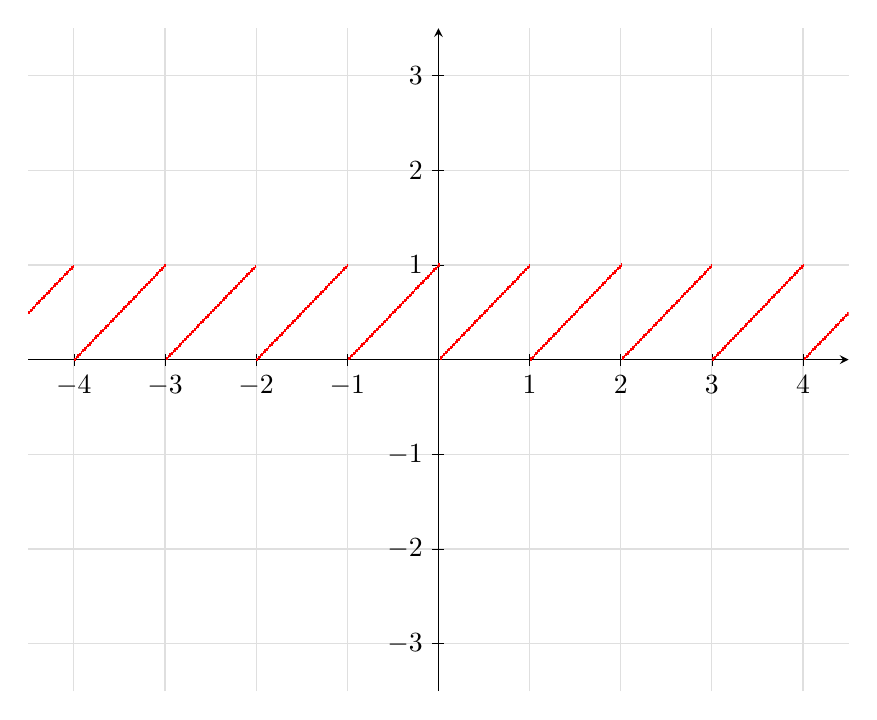
\begin{tikzpicture}
            \begin{axis}[
                axis lines=middle,
                xlabel={},
                ylabel={},
                xtick={-4,-3,...,4},
                ytick={-3,-2,...,3},
                xmin=-4.5, xmax=4.5,
                ymin=-3.5, ymax=3.5,
                width=12cm,
                height=10cm,
                grid=major,
                grid style={thin, lightgray!50},
                tick style={black},
                minor tick num=0,
            ]
            \addplot[
                domain=-4.5:4.5,
                samples=501, 
                very thick,
                red,
                jump mark left, 
                unbounded coords=jump,
            ] {x - floor(x)};
            \end{axis}
        \end{tikzpicture}
        }
    \end{center}
\end{example}

\begin{definition}{}{def_2_3_5}
    \textbf{Implicit representation of a function} refers to defining the relationship between the variables without explicitly solving for one variable in terms of the other.
    \[
    \sin (xy) - x^{2} + y = 1
    \]
\end{definition}

\begin{definition}{}{}
    \textbf{Parametric representation of a function} refers to expressing the dependent and independent variables of a function using one or more parameters.
    \[
    x(t) = \cos t, \quad y(t) = \sin(t), \quad t\in [0, 2\pi]
    \]
\end{definition}

\begin{definition}{}{}
    \textbf{Graphical representation of a function} refers to visualizing the relationship between the independent variable and the dependent variable on a coordinate plane or graph.
\end{definition}

\begin{definition}{}{}
    \textbf{Numerical representation of a function} refers to expressing the function using a table of values that show specific input-output pairs.
    \[
        \begin{array}{c|c}
            x & f(x) \\
            \hline
            -2 & 4 \\
            -1 & 1 \\
            0 & 0 \\
            1 & 1 \\
            2 & 4 \\
        \end{array}
    \]
\end{definition}

\begin{definition}{}{}
    \textbf{Mapping representation of a function} refers to describing the function as a relationship that assigns each element from the domain (input set) to a unique element in the codomain (output set).
    \[
        f: \{1, 2, 3\} \to \{a, b, c\}, \quad f(1) = a, \quad f(2) = b, \quad f(3) = c
    \]    
    \[
        \text{Domain} \quad 1 \longrightarrow a, \quad 2 \longrightarrow b, \quad 3 \longrightarrow c \quad \text{(Codomain)}
    \]
\end{definition}



\subsection{Basics Properties of Functions}
There are various properties of functions, including boundedness, monotonicity, parity, continuity, differentiability, periodicity, convexity and concavity, and etc.
\begin{enumerate}
    \item[1.]\textbf{Boundedness}
\begin{definition}{}{def_2_3_10}
    A function $f$ is \textbf{bounded} if and only if there exists $m < M, \, m, M \in \mathbb{R}$ such that $m \leq f(x) \leq M$, for all $\, x \in D_{f}$. Here, $m$ is called a \textbf{lower bound} and $M$ is called an \textbf{upper bound}.
\end{definition}

\noindent The following definition is equivalent to the Definition \ref{:def_2_3_10}.

\begin{definition}{}{}
    A function $f$ is \textbf{bounded} if and only if $ \exists \, X \in \mathbb{R}$ such that $\vert f(x) \vert \leq X, \text{ for all } x \in D_{f}$.
\end{definition}
\begin{note}
    If a function $f$ is bounded, its lower and upper bounds are non-unique.
\end{note}

\item[2.] \textbf{Monotonicity}
\begin{definition}{}{}
    For any $x_{1}, x_{2} \in D_{f}$, if we have $ x_{1} < x_{2} \implies f(x_{1}) \leq f(x_{2})$ or $f(x_{1}) < f(x_{2})$, then we say the function $f$ is \textbf{monotonic increasing} or \textbf{strictly increasing}. We denoted it as $f(x) \uparrow$.  
\end{definition}

\begin{definition}{}{}
    For any $x_{1}, x_{2} \in D_{f}$, if we have $ x_{1} < x_{2} \implies f(x_{1}) \geq f(x_{2})$ or $f(x_{1}) > f(x_{2})$, then we say the function $f$ is \textbf{monotonic decreasing} or \textbf{strictly decreasing}. We denoted it as $f(x) \downarrow$. 
\end{definition}

\begin{example}{}{}
    \textcolor{red}{give some simple examples}     
\end{example}

\item[3.] \textbf{Parity}
\begin{definition}{}{}
    A function $f$ is called an \textbf{even function} if it satisfies the condition:
    \[
    f(x) = f(-x), \forall x \in D_{f}.
    \]
\end{definition}
\begin{note}
    This means the function is symmetric with respect to the $y$-axis.
\end{note}

\begin{definition}{}{}
    A function $f$ is called an \textbf{odd function} if it satisfies the condition:
    \[
    f(x) = -f(-x), \forall x \in D_{f}.
    \]
\end{definition}
\begin{note}
    This means the function has rotational symmetry about the origin ($180-$degree rotation).
\end{note}

\begin{example}{}{}
    \textcolor{red}{Give some simple examples.}
\end{example}

\item[4.] \textbf{Periodicity}
\begin{definition}{}{}
    A function $f$ is said to be \textbf{periodic} if there exists a positive constant $T$ such that:
    \[
    f(x+T) = f(x), \forall x\in D_{f}.
    \]
    The \textcolor{red}{smallest, positive} constant $T$ is called the \textbf{period} of the function. 
\end{definition}
\begin{example}{}{}
    \textcolor{red}{give some simple examples.}
\end{example}
\begin{note}
    This means that the function repeats its values in regular intervals, and $T$ is the \textcolor{red}{smallest} such interval where the function's values begin to repeat.
\end{note}

\begin{example}{}{}
    Do all periodic functions have a smallest period? \\
    The \textbf{Dirichlet function} is 
    \[
        D(x) =
        \begin{cases}
              0, & \text{if } x \in \mathbb{R} \setminus \mathbb{Q}, \\
              1, & \text{if } x \in \mathbb{Q}.
        \end{cases}
    \]
    It should be obvious that any $T \in \mathbb{Q}^{+}$ makes the Dirichlet function a periodic function, so it is a period function without a period (\textcolor{red}{smallest, positive} $T$).
\end{example}
 
\end{enumerate}



\section{Some Useful Inequalities and Identities}
\begin{proposition}{}{prop_2_4_1}
    For all $x \in \mathbb{R}$, we have that 

    \begin{enumerate}[topsep=10pt, itemsep=5pt]
        \item $\vert x\vert \geq 0$ with $\vert x \vert = 0$, iff $x=0$. 
        \item $\vert xy \vert = \vert x \vert \vert y \vert $.
        \item $\vert x^{2} \vert = \vert x \vert^{2} = x^{2}$. 
    \end{enumerate}
\end{proposition}
\begin{proposition}{}{prop_2_4_2}
    \textbf{The Triangle Inequality}. For any $a, b \, \in \mathbb{R}$, we have 
    \[
    \big\vert \vert a \vert - \vert b \vert \big\vert \leq \vert a + b \vert \leq \vert a \vert + \vert b \vert.
    \]
\end{proposition}
\begin{proof}{MyPropColor}
    \begin{align*}
        - 2\vert a \vert \vert b \vert &\leq 2ab \leq 2\vert a \vert \vert b \vert \\
        a^{2} - 2\vert a \vert \vert b \vert + b^{2} &\leq a^{2} + 2ab + b^{2} \leq a^{2} + 2\vert a \vert \vert b \vert + b^{2} \\
        \left( \vert a \vert - \vert b \vert\right)^2 &\leq (a+b)^{2} \leq \left( \vert a \vert + \vert b \vert\right)^2 \\
        \big\vert \vert a \vert - \vert b \vert \big\vert &\overset{(1)}{\leq} \vert a + b \vert \overset{(2)}{\leq} \vert a \vert + \vert b \vert.
    \end{align*}
    
    Here, the inequality $(1)$ means that one side of the triangle is greater than the difference between the other two sides, and the inequality $(2)$ means that the sum of two sides of a triangle is greater than the third side.
\end{proof}
The triangle inequality is used extensively in analysis.

\begin{definition}{}{}
    The \textbf{Arithmetic Mean (AM)} is: 
    \[
        \frac{a_{1} + a_{2} + \dots + a_{n}}{n}
    \]
\end{definition}

\begin{definition}{}{}
    The \textbf{Geometric Mean (GM)} is:
    \[
        \sqrt[n]{a_{1}a_{2}\dots a_{n}}
    \]
\end{definition}

\begin{definition}{}{}
    The \textbf{Harmonic Mean (HM)} is:
    \[
        \frac{n}{\frac{1}{a_{1}} + \frac{1}{a_{2}} + \dots + \frac{1}{a_{n}}}
    \]
\end{definition}

\begin{proposition}{}{prop_2_4_£}
\textbf{AM-GM-HM Inequality}: 
\[
    \frac{a_{1} + a_{2} + \dots + a_{n}}{n} \quad \overset{(1)}{\geq} \quad  \sqrt[n]{a_{1}a_{2}\dots a_{n}} \quad \overset{(2)}{\geq} \quad \frac{n}{\frac{1}{a_{1}} + \frac{1}{a_{2}} + \dots + \frac{1}{a_{n}}}
\]
\end{proposition}
\begin{proof}{MyPropColor}
    To prove inequality $(1)$. It is obvious that $n= 1, 2$ the inequality $(1)$ holds. For $n=4$, $\frac{a_{1}+a_{2}+a_{3}+a_{4}}{4} \geq \frac{2\cdot\sqrt{a_{1}a_{2}} + 2\cdot\sqrt{a_{3}a_{4}}}{4} = \frac{\sqrt{a_{1}a_{2}} + \sqrt{a_{3}a_{4}}}{2} \overset{(3)}{\geq} \sqrt[4]{a_{1}a_{2}a_{3}a_{4}}$. In the inequality $(3)$, we apply the AM $\geq$ GM for $n=2$. In other words, we view $\sqrt{a_{1}a_{2}}$ and $\sqrt{a_{3}a_{4}}$ as $b_{1}, b_{2}$, respectively. Thus, we have shown that when $n = 2^{k}, k \in \mathbb{N}$, the inequality $(1)$ holds. Now, if $n \neq 2^{k}$, then $\exists\, l \in \mathbb{N}$ s.t. $2^{l-1} < n < 2{l}$. Let $\sqrt[n]{a_{1}a_{2}a_{3}\dots a_{n}} = \bar{a}$, we composite the sequence below
    \[
        a_{1}, a_{2}, a_{3}, \dots, a_{n}, \underbrace{\bar{a}, \bar{a}, \dots, \bar{a}}_{2^{l} - n\text{ number of } \bar{a}}.
    \]
    Then, we have
    \begin{align*}
    \frac{a_{1} + a_{2} + \dots + a_{n} + (2^{l}-n)\bar{a}}{2^{l}}
    &\ge \sqrt[2^{l}]{a_{1}a_{2}\dots a_{n}\bar{a}\bar{a}\dots \bar{a}} \\[4pt]
    &= \sqrt[2^{l}]{\bar{a}^{n}\cdot \bar{a}^{2^{l}-n}} \\
    &= \sqrt[2^{l}]{\bar{a}^{2^{l}}} \\
    &= \bar{a}.
    \end{align*}
    That is 
    \begin{align*}
        \frac{a_{1} + a_{2} + a_{3} + \dots + a_{n} + (2^{l}-n)\cdot\bar{a}}{2^{l}} &\geq \bar{a} \\
        a_{1} + a_{2} + a_{3} + \dots + a_{n} + (2^{l}-n)\cdot \bar{a} &\geq 2^{l}\bar{a} \\
        a_{1} + a_{2} + a_{3} + \dots + a_{n} &\geq n\bar{a} \\
        \frac{a_{1} + a_{2} + a_{3} + \dots + a_{n}}{n} &\geq \bar{a} \\
        \frac{a_{1} + a_{2} + a_{3} + \dots + a_{n}}{n} &\geq \sqrt[n]{a_{1}a_{2}a_{3}\dots a_{n}}.
    \end{align*}
    This completes the proof of the inequality $(1)$.
    
    To prove inequality $(2)$, we replace $a_{i}$, with $\frac{1}{a_{i}}$, for $i \in \{1, 2, 3, \dots, n\}$ and repeat the process above.
\end{proof}


\begin{proposition}{}{prop_2_4_4}
\textbf{Pascal's Triangle Identity.} For $n,k \in \mathbb{N}$ with $2 \leq k \leq n$ we have that 
\[
\binom{n}{k-1} + \binom{n}{k} = \binom{n+1}{k}.
\]
\end{proposition}
\begin{proof}{MyPropColor}
    We have
    \begin{align*}
        \binom{n}{k-1} + \binom{n}{k} &= \frac{n
        !}{\big(n-(k-1)\big)!(k-1)!} + \frac{n!}{(n-k)!k!} \\
        &= \frac{n(n-1)\cdots \big(n-(k-1) + 1\big)}{(k-1)!} + \frac{n(n-1)\cdots (n-k+1)}{k!} \\
        &= \frac{n(n-1)\cdots (n- k + 2)}{(k-1)!} + \frac{n(n-1)\cdots (n-k+1)}{k!} \\
        &= \frac{kn(n-1)\cdots (n- k + 2)}{k!} + \frac{n(n-1)\cdots (n-k+1)}{k!} \\
        &= \frac{kn(n-1)\cdots (n- k + 2)}{k!} + \frac{n(n-1)\cdots (n-k+2)(n-k+1)}{k!} \\
        &= \frac{n(n-1)\cdots(n-k+2)}{k!}\cdot\big(k+(n-k+1)\big) \\
        &= \frac{n(n-1)\cdots(n-k+2)}{k!}\cdot(n+1) \\
        &= \frac{(n+1)n(n-1)\cdots(n-k+2)}{k!} \\
        &= \frac{(n+1)n(n-1)\cdots\big((n+1)-k+1\big)}{k!} \\
        &= \frac{(n+1)!}{\big((n+1)-k\big)!k!} = \binom{n+1}{k}
    \end{align*}
\end{proof}


\begin{proposition}{}{prop_2_4_5}
    \textbf{Binomial Theorem.} For $x, y \in \mathbb{R}$ and $n \in \mathbb{N}$, we have that
    \[
        (x+y)^{n} = \sum\limits_{k=0}^{\textcolor{red}{k=}n}\binom{n}{k}x^{n-k}y^{k}.
    \]
\end{proposition}
\begin{proof}{MyPropColor}
    We prove the binomial theorem by Mathematical Induction. 

    Base case: $n=0$, it is easy to see that $LHS = RHS$. 

    Hypothesis: As long as 
    \[
        (x+y)^{m} = \sum\limits_{k=0}^{\textcolor{red}{k=}m}\binom{m}{k}x^{m-k}y^{k}, \quad\forall \,m \in \mathbb{N}, m \leq n-1,
    \] 
    then we prove that 
    \[
        (x+y)^{m+1} = \sum\limits_{k=0}^{\textcolor{red}{k=}m+1}\binom{m+1}{k}x^{m+1-k}y^{k}
    \]
    still holds. 
    \begin{align*}
        (x+y)^{m+1} &= (x+y)(x+y)^{m} \\
        &= (x+y)\sum\limits_{k=0}^{\textcolor{red}{k=}m}\binom{m}{k}x^{m-k}y^{k}. \\
        &= \sum\limits_{k=0}^{m}\binom{m}{k}x^{m-k+1}y^{k} + \sum\limits_{k=0}^{m}\binom{m}{k}x^{m-k}y^{k+1} \\
        &= \sum\limits_{k=0}^{m}\binom{m}{k}x^{m-k+1}y^{k} + \sum\limits_{k-1=0}^{k-1= m}\binom{m}{k-1}x^{m-(k-1)}y^{(k-1)+1} \\
        &= \sum\limits_{k=0}^{m}\binom{m}{k}x^{m-k+1}y^{k} + \sum\limits_{k=1}^{k= m+1}\binom{m}{k-1}x^{m-k+1}y^{k} \\
        &= x^{m+1} + \sum\limits_{k=1}^{m}\binom{m}{k}x^{m-k+1}y^{k} + \sum\limits_{k=1}^{k= m}\binom{m}{k-1}x^{m-k+1}y^{k} + y^{m+1} \\
        &= x^{m+1} + \sum\limits_{k=1}^{m} \left[\binom{m}{k} + \binom{m}{k-1}\right]x^{m-k+1}y^{k} + y^{m+1} \\
        &= x^{m+1} + \sum\limits_{k=1}^{m} \binom{m+1}{k}x^{m-k+1}y^{k} + y^{m+1} \\
        &= \binom{m+1}{0}x^{m+1} + \sum\limits_{k=1}^{m} \binom{m+1}{k}x^{m-k+1}y^{k} + \binom{m+1}{m+1}y^{m+1} \\
        &= \sum\limits_{k=0}^{m+1}\binom{m+1}{k}x^{m+1-k}y^{k}.
    \end{align*}
\end{proof}


\begin{proposition}{\quad}{prop_2_4_6}
    Show that $0.\dot{9} = 0.999\dots = 1$.
\end{proposition}

\begin{proof}{MyPropColor}
    We treat $0.999\dots$ as the sum of a geometric series:
    \begin{align*}
        0.999\dots &= 0.9 + 0.09 + 0.009 + \dots
    \end{align*}
    This series has a sum given by:
    \[
    S = \frac{a}{1-r} = \frac{0.9}{1-0.1} = \frac{0.9}{0.9} = 1.
    \]
\end{proof}